% Provenance (never printed): see sources/outline_sources.md (Year 3:
% geomorphology, hillslope processes, river incision, landscape evolution).
% Brief: sources/book5/BRIEFS.md, ch. 18. Curves from
% figdata/bachelor-3/hillslope.py, stream_profile.py and varden_river.py.
% Exercise and problem values in the Book 5 scratch calculator calc/ch18.py.
% The upland west of the Varden Hills, its river, its tributaries, its
% uplift rate and its base-level fall are invented; the outlet elevation is
% the region model's river at the west edge of the map.
\chapter{定量地貌学}\label{ch:b3:quantitative-geomorphology}

河流穿越正在隆升的山脉时，纵剖面上会出现一处台阶：瀑布，
其下方为峡谷，上方为较平缓的河谷。这一台阶并不会
停留在形成的位置。它向上游迁移，速率为每年几毫米或几米，
其位置是一座计时钟，计时始于河流的\omterm{def:b3:quantitative-geomorphology:knickpoint}{侵蚀基准面}
被降低之时。读出这座钟，以及写在山丘与河流形貌中的速率，
需要两条守恒定律和两条输运定律：一条描述沿坡蠕动的土壤，
另一条描述河流切割的基岩。

\begin{recall}
风化、侵蚀、沉积、地貌，以及隆升与侵蚀之间的平衡，
均衡回弹与U形
冰川谷，均见于中学课本。剥蚀速率、床面剪应力与希尔兹
参数见于本科一年级分册中关于侵蚀与输运的一章；
数字高程模型见于其中关于地质图的一章；艾里
均衡见于其中关于均衡与重力异常的一章。\omterm{def:b3:advanced-geochronology:cosmogenic}{宇宙成因
核素}及由其导出的侵蚀速率见于
第~\ref{ch:b3:advanced-geochronology}~章，\omterm{def:b3:orogenic-wedges:thermochronology}{热年代学}与
\omterm{def:b3:orogenic-wedges:age-elevation}{年龄–高程关系}见于第~\ref{ch:b3:orogenic-wedges}~章。
扩散方程见于物理学教材。
\end{recall}

\section{坡面}\label{sec:b3:quantitative-geomorphology:hillslopes}

在覆盖土壤的山坡上，土壤沿坡向下逐粒移动：穴居
动物将其抛出，根系将其顶起，凝固与润湿使其膨胀，每一次
扰动都使重力将其稍作移动。若按世纪平均，土壤的
通量与坡度成正比。

\begin{definition}[坡面扩散]\label{def:b3:quantitative-geomorphology:diffusion}
称\emph{坡面扩散}\index{坡面扩散}为土壤沿坡向下的缓慢输运，
其单位坡宽的土壤体积通量，
即 $\vec q$，与地表高程 $z$ 的梯度成正比：
$\vec q = -\kappa\,\nabla z$。系数 $\kappa$ 的单位为
\unit{m^2/\text{年}}，称为坡面扩散系数。
\end{definition}

\begin{theorem}[坡面的扩散]\label{thm:b3:quantitative-geomorphology:diffusion}
设岩石相对于界定该坡面的河道以速率 $U$ 隆升，
土壤与岩石密度相同，且土壤以\omterm{def:b3:quantitative-geomorphology:diffusion}{坡面
扩散}方式移动，$\kappa$ 处处均匀。于是地表高程满足
\[
\frac{\partial z}{\partial t} = U + \kappa\,\nabla^2 z ,
\]
这是带源项的扩散方程。
\end{theorem}

\begin{proof}
取坡面上一小块面积 $\delta S$，其体积变化包括隆升，
即单位时间增加 $U\,\delta S$，另有经边界流出的土壤，
其量为 $\oint \vec q\cdot\vec n\,\mathrm{d}\ell = (\nabla\cdot\vec q)\,\delta S$。
由此得 $\partial z/\partial t = U - \nabla\cdot\vec q$；代入 $\vec q = -\kappa
\nabla z$ 且 $\kappa$ 均匀，则 $\nabla\cdot\vec q = -\kappa\nabla^2 z$。
\end{proof}

断层或海岸线在某一时刻切出陡坎；此后陡坎只
进行扩散。设半高为 $a$ 的竖直台阶位于远场坡度为 $b$ 的斜坡上，
一维情形下其解为
\[
z(x,t) = a\,\operatorname{erf}\!\left(\frac{x}{2\sqrt{\kappa t}}\right) + b\,x ,
\qquad
\left.\frac{\partial z}{\partial x}\right|_{x=0} = \frac{a}{\sqrt{\pi\kappa t}} + b .
\]
形状仅取决于乘积 $\kappa t$：实测剖面给出
$\kappa t$，若另有独立年龄，可得 $\kappa$；若已知 $\kappa$，
则可得年龄，即\emph{形态年龄}。半干旱地区、土壤呈颗粒状且植被稀疏的陡坎，
所得 $\kappa$ 介于
$10^{-3}$ 与 \qty{e-2}{m^2/\text{年}} 之间；湿润、植被茂密的沿海山地
约为 \qty{5e-3}{m^2/\text{年}}。
% ledger: whipple04:scarp-erf, whipple04:scarp-kappa

\begin{omfigure}
\begin{tikzpicture}
\begin{groupplot}[group style={group size=2 by 1, horizontal sep=1.6cm},
  width=0.48\linewidth, height=0.36\linewidth, tick label style={font=\scriptsize},
  label style={font=\small}, legend style={font=\scriptsize, draw=none, fill=none}]
\nextgroupplot[xlabel={距离 $x$ (m)}, ylabel={$z$ (m)}, xmin=-40, xmax=40,
  ymin=-5, ymax=5, legend pos=north west]
% computed in figdata/bachelor-3/hillslope.py
\addplot[black!50, densely dashed] table[x=x, y=z0] {figdata/out/bachelor-3-hillslope-scarp.dat};
\addplot[omDef, thick] table[x=x, y=z1] {figdata/out/bachelor-3-hillslope-scarp.dat};
\addplot[omProp, thick] table[x=x, y=z2] {figdata/out/bachelor-3-hillslope-scarp.dat};
\addplot[omThm, thick] table[x=x, y=z3] {figdata/out/bachelor-3-hillslope-scarp.dat};
\legend{初始, \qty{2}{ka}, \qty{10}{ka}, \qty{40}{ka}}
\nextgroupplot[xlabel={距分水岭的距离 (m)}, ylabel={高度 (m)},
  xmin=-150, xmax=150, ymin=0, ymax=200, xtick={-150,-75,0,75,150}]
\addplot[omMeth, thick] table[x=x, y=z1] {figdata/out/bachelor-3-hillslope-hill.dat};
\addplot[omDef, thick] table[x=x, y=z2] {figdata/out/bachelor-3-hillslope-hill.dat};
\addplot[omThm, thick] table[x=x, y=z3] {figdata/out/bachelor-3-hillslope-hill.dat};
\node[font=\scriptsize, anchor=north] at (axis cs:0,45) {0.0215};
\node[font=\scriptsize, anchor=north] at (axis cs:0,94) {0.043};
\node[font=\scriptsize, anchor=north] at (axis cs:0,184) {\qty{0.086}{mm/\text{年}}};
\end{groupplot}
\end{tikzpicture}

\par\smallskip{\small 左图：陡坎偏移 \qty{5}{m}，位于坡度为
0.05 的斜坡上，以 $\kappa = \qty{5e-3}{m^2/\text{年}}$ 扩散：初始台阶
（虚线）以及经过 2、10 和 \qty{40}{ka} 后的剖面。右图：
处于\omterm{def:b3:quantitative-geomorphology:steady-profile}{稳态}的山丘，半宽 \qty{150}{m}，$\kappa$ 相同（高度自
河道算起），降低速率分别为
0.0215、0.043 和 \qty{0.086}{mm/\text{年}}：抛物线形，其起伏与山顶
曲率均与剥蚀速率成正比。}\label{fig:b3:quantitative-geomorphology:hillslope}
\end{omfigure}
% ledger: whipple04:scarp-kappa

当一座山丘经历足够长时间的抬升与剥蚀后，
其形状便不再变化：每一点降低的速率恰好等于岩石上升的速率。

\begin{proposition}[山顶曲率量度剥蚀速率]\label{prop:b3:quantitative-geomorphology:curvature}
在\omterm{def:b3:quantitative-geomorphology:diffusion}{坡面扩散}作用下处于\omterm{def:b3:quantitative-geomorphology:steady-profile}{稳态}的山坡上，
剥蚀速率 $E$ 等于 $U$，满足
\[
E = -\kappa\,\nabla^2 z .
\]
一维情形下，剖面为抛物线 $z = z_0 - E x^2/(2\kappa)$，
分水岭与河道之间的起伏为 $E L^2/(2\kappa)$，二者
相距 $L$。
\end{proposition}

\begin{proof}
在定理中令 $\partial z/\partial t = 0$，得 $\kappa\nabla^2 z =
-U = -E$。一维情形下，两次积分并取 $\mathrm{d}z/\mathrm{d}x =
0$（于分水岭处），即得抛物线，其在 $x = L$ 处的值即为起伏。
\end{proof}

曲率是在数字高程模型上测得的几何量，因此
一旦知道 $\kappa$，它便可解读为速率：山顶越陡、曲率越大，
景观剥蚀得越快。土壤本身由下方的岩石形成，
其速率取决于土层已覆盖的厚度。

\begin{definition}[土壤生成函数]\label{def:b3:quantitative-geomorphology:soil-production}
\emph{土壤生成函数}\index{土壤生成函数}给出
基岩转化为土壤的速率 $P$ 与
土层厚度 $h$ 的函数关系；通常取 $P = P_0\,e^{-h/h_0}$，其中
$P_0$ 为裸岩上的速率，$h_0$ 为几分之一米量级的长度。
\end{definition}

\omterm{def:b3:quantitative-geomorphology:steady-profile}{稳态}时，土壤与岩石的界面以与地表相同的速率降低，
即 $P(h) = E$，于是土层厚度为 $h = h_0 \ln(P_0/E)$：剥蚀越快，
土层越薄；当 $E$ 超过 $P_0$ 时，土壤被剥离，
裸露的岩石因风化受限而出露。实测到的最快土壤生成速率
约为 \qty{0.5}{mm/\text{年}}。
% ledger: whipple04:soil

线性扩散在陡坡上失效。当坡度接近某一
阈值时，颗粒以阵发的方式滚动、滑移，浅层滑坡
剥离土壤。

\begin{definition}[临界坡度]\label{def:b3:quantitative-geomorphology:critical}
\emph{临界坡度}\index{临界坡度}
$S_c$ 为土壤通量无限增长时的坡度；
在一种广泛使用的非线性输运定律中，$q = \kappa S/[1 - (S/S_c)^2]$。
\end{definition}

坡度远小于 $S_c$ 的斜坡表现如线性扩散；剥蚀较快的斜坡
则逐渐变陡并趋向 $S_c$，变得近于平直，其坡度
由阈值而非剥蚀速率决定。
% ledger: whipple04:nonlinear

\begin{inthefield}[扫描山坡]
一支测绘队在一条覆有土层的山脊上工作，将地面激光扫描仪
架设在距山脊顶部几十米处的三脚架上。每次扫描记录数百万个
点，即透过草丛与灌木间的空隙测得的到地面的距离与方向；
多个扫描站的点被合并
为一个点云，并以卫星接收机测量的标靶进行配准，
保留最后一次回波以去除植被。裸地点云
被划分为分米级网格，构成高程模型，并平滑约几米，
并在山脊顶部计算其拉普拉斯算子。随后，队伍比较
以\omterm{def:b3:advanced-geochronology:cosmogenic}{宇宙成因核素}测得剥蚀速率的各山脊的山顶曲率：
将二者相互作图，其给出的山坡扩散系数表现为
直线的斜率，正如该命题所预言的。
\end{inthefield}

\section{河流下切}\label{sec:b3:quantitative-geomorphology:rivers}

河流流经基岩时，通过拔取岩块、
借推移质的磨蚀以及空穴化作用而下切。这些过程均与
水流施加于河床的切应力，或其在此耗散的功率成比例，二者均随
流量与坡度增大而增大。流量随汇水面积增大，因此面积可代表
流量。

\begin{definition}[河流功率定律]\label{def:b3:quantitative-geomorphology:stream-power}
\emph{河流功率定律}\index{河流功率定律}给出基岩河流的
垂直下切速率 $E$ 为
\[
E = K A^m S^n ,
\]
其中 $A$ 为该点上游的汇水面积，$S$ 为河道
坡度，$m$ 与 $n$ 为正指数，$K$ 为可蚀性系数，
它综合反映岩石强度、气候与河道宽度。
\end{definition}

对于与切应力或单位河流功率成比例的过程，
$m/n$ 接近 0.5。对软弱岩层中切割而成的荒地河道
为期约 20 年的调查发现，下切速率与 $A^{0.44}S^{0.68}$ 成正比。
% ledger: whipple04:spim

\begin{definition}[剥离限制型与搬运限制型下切]\label{def:b3:quantitative-geomorphology:limited}
下切为\emph{剥离限制型}\index{剥离限制型下切}，
当河流能够带走的泥沙多于其所获得的泥沙时，其下降速率
取决于河流将基岩从河床上剥离的快慢：
适用\omterm{def:b3:quantitative-geomorphology:stream-power}{河流功率定律}。当河流携带其所能携带的全部泥沙时，下切为
\emph{搬运限制型}\index{搬运限制型下切}，其河床仅在
输沙能力沿下游增大之处才降低，
降低速率由
泥沙通量的散度决定。
\end{definition}

\omterm{def:b3:quantitative-geomorphology:limited}{搬运限制型}河流的行为与山坡颇为相似：通量取决于
坡度，其剖面按一类扩散方程演化，将
任何台阶磨圆。\omterm{def:b3:quantitative-geomorphology:limited}{剥离限制型}河流则保持台阶锐利并使其
移动，下一节将予以说明。基岩河床且仅覆有薄层砾石的山地河流
通常更接近前者；覆有厚层冲积物的河流则
更接近后者。

\begin{omfigure}
\begin{tikzpicture}[x=0.55cm, y=0.55cm, font=\scriptsize,
  declare function={f(\x)=2.1+3.5*(1-(\x-0.5)/10)^2;
    tl(\x,\l)=f(\x)-1.1*exp(-(10.5-\x)/\l);}]
\begin{scope}
\draw[->] (0,0) -- (11.5,0) node[below left] {距下游距离};
\draw[->] (0,0) -- (0,6) node[above right] {$z$};
\draw[black!50, densely dashed] plot[domain=0.5:10.5, samples=40] (\x,{f(\x)});
\draw[omDef, thick] plot[domain=0.5:6.5, samples=30] (\x,{f(\x)}) -- plot[domain=6.5:10.5, samples=20] (\x,{f(\x)-1.1});
\draw[omThm, thick] plot[domain=0.5:3.5, samples=20] (\x,{f(\x)}) -- plot[domain=3.5:10.5, samples=30] (\x,{f(\x)-1.1});
\draw[->, black!70] (6.3,4.1) -- (3.8,4.75);
\node[anchor=west, align=left] at (5.6,5.3) {剥离限制型：\\ 台阶向上游移动};
\node at (5.5,-0.7) {(a)};
\end{scope}
\begin{scope}[xshift=7.2cm]
\draw[->] (0,0) -- (11.5,0) node[below left] {距下游距离};
\draw[->] (0,0) -- (0,6) node[above right] {$z$};
\draw[black!50, densely dashed] plot[domain=0.5:10.5, samples=40] (\x,{f(\x)});
\draw[omDef, thick] plot[domain=0.5:10.5, samples=40] (\x,{tl(\x,1.2)});
\draw[omThm, thick] plot[domain=0.5:10.5, samples=40] (\x,{tl(\x,3.5)});
\node[anchor=west, align=left] at (5.0,5.3) {搬运限制型：\\ 下降向上游扩散};
\node at (5.5,-0.7) {(b)};
\end{scope}
\end{tikzpicture}

\par\smallskip{\small 河流对\omterm{def:b3:quantitative-geomorphology:knickpoint}{侵蚀基准面}下降的响应
（虚线：下降前的剖面；蓝色、红色分别为之后的两个时刻），
示意图。(a) \omterm{def:b3:quantitative-geomorphology:limited}{剥离限制型}河流保持一个锐利的\omterm{def:b3:quantitative-geomorphology:knickpoint}{裂点}，
该\omterm{def:b3:quantitative-geomorphology:knickpoint}{裂点}向上游迁移；\omterm{def:b3:quantitative-geomorphology:knickpoint}{裂点}下方的剖面保持原有形状，仅整体下降。(b) \omterm{def:b3:quantitative-geomorphology:limited}{搬运限制型}
河流逐步降低其整个剖面，降幅在靠近
出口处最大。}\label{fig:b3:quantitative-geomorphology:regimes}
\end{omfigure}

若岩石相对于河流出口以均匀速率 $U$ 上升，且 $K$，
$m$、$n$ 均为常数，则河流演化满足 $\partial z/\partial t = U - K A^m
S^n$。

\begin{definition}[稳态河流剖面]\label{def:b3:quantitative-geomorphology:steady-profile}
当河流剖面的高程不再随时间变化时，称其处于\emph{稳态}\index{稳态}，
即在每一点，下切量都与
岩石相对于出口的隆升量相平衡。
\end{definition}

\begin{theorem}[河流功率定律下的稳态剖面]\label{thm:b3:quantitative-geomorphology:steady}
在 $U$、$K$、$m$、$n$ 均为常数的条件下，\omterm{def:b3:quantitative-geomorphology:limited}{剥离限制型}河流处于
\omterm{def:b3:quantitative-geomorphology:steady-profile}{稳态}时，其坡度满足
\[
S = \left(\frac{U}{K}\right)^{1/n} A^{-m/n} .
\]
\end{theorem}

\begin{proof}
\omterm{def:b3:quantitative-geomorphology:steady-profile}{稳态}时 $\partial z/\partial t = 0$，故 $K A^m S^n = U$，从而 $S^n
= (U/K)A^{-m}$；两边取 $n$ 次方根即得结论。
\end{proof}

\begin{omfigure}
\begin{tikzpicture}
\begin{groupplot}[group style={group size=2 by 1, horizontal sep=1.7cm},
  width=0.48\linewidth, height=0.33\linewidth, tick label style={font=\scriptsize},
  label style={font=\small}]
\nextgroupplot[xlabel={距分水岭距离 (km)}, ylabel={$z$ (m)},
  xmin=0, xmax=12, ymin=150, ymax=420]
% computed in figdata/bachelor-3/stream_profile.py
\addplot[omDef, thick] table[x=d, y=z] {figdata/out/bachelor-3-stream_profile-steady.dat};
\nextgroupplot[xmode=log, ymode=log, xlabel={汇水面积 $A$ (\unit{km^2})},
  ylabel={坡度 $S$}, xmin=0.1, xmax=100, ymin=0.003, ymax=0.2]
\addplot[omDef, thick] table[x=A, y=S] {figdata/out/bachelor-3-stream_profile-steady.dat};
\addplot[only marks, mark=*, mark size=1.4pt, omThm] table[x=A, y=S] {figdata/out/bachelor-3-stream_profile-sa.dat};
\addplot[omThm, densely dashed] table[x=A, y=S] {figdata/out/bachelor-3-stream_profile-fit.dat};
\end{groupplot}
\end{tikzpicture}

\par\smallskip{\small 瓦尔登丘陵以西虚构山地河流的\omterm{def:b3:quantitative-geomorphology:steady-profile}{稳态}剖面
（$U = \qty{0.043}{mm/\text{年}}$，$K =
\qty{e-6}{\text{年}^{-1}}$，$m = 0.5$，$n = 1$），自河道源头
至海拔 \qty{170}{m} 的出口。右图为坡度随面积的变化：模型（蓝线）
与在 \qty{200}{m} 河段上测得的十二个坡度
（红点，散布约 \qty{10}{\percent}），其最小二乘直线
（虚线）斜率为 $-0.47$。}\label{fig:b3:quantitative-geomorphology:profile}
\end{omfigure}

坡度随面积按幂律递减，剖面呈上凹形。
即使定理的假设存疑，实际河流仍常服从此类幂律，
因此两个数即可概括一条剖面。
% ledger: whipple04:steepness

\begin{definition}[河道陡峭指数与凹度指数]\label{def:b3:quantitative-geomorphology:indices}
当河流坡度满足 $S = k_s A^{-\theta}$ 时，
指数 $\theta$ 称为\emph{凹度指数}\index{凹度指数}，系数
$k_s$ 称为\emph{河道陡峭指数}\index{河道陡峭指数}。
为便于比较河流，将 $\theta$ 统一取为参考值
$\theta_{\mathrm{ref}}$，并称 $k_{sn} = S A^{\theta_{\mathrm{ref}}}$
为标准化陡峭指数。
\end{definition}

由定理可知 $\theta = m/n$，$k_s = (U/K)^{1/n}$：
在给定侵蚀性下，岩石隆升越快，河流越陡。
因此，山脉的陡峭指数图可勾勒出其隆升格局。


坡度是带噪声高程的导数，散布很大。
改对剖面积分，所用高程测量更可靠。

\begin{definition}[Chi 分析]\label{def:b3:quantitative-geomorphology:chi}
\emph{Chi 分析}\index{Chi 分析}将河网中各点的高程
对下述坐标作图，
\[
\chi(x) = \int_{x_b}^{x} \left(\frac{A_0}{A(x')}\right)^{\theta}
\mathrm{d}x' ,
\]
其中 $x$ 为沿河道自基点
$x_b$ 向上游的距离，$A_0$ 为参考面积，$\theta$ 为\omterm{def:b3:quantitative-geomorphology:indices}{凹度指数}；
$\chi$ 的量纲为长度。
\end{definition}

\begin{proposition}[chi 变换将稳态剖面拉直]\label{prop:b3:quantitative-geomorphology:chi}
在\omterm{def:b3:quantitative-geomorphology:steady-profile}{稳态}定理的假设下，取 $\theta = m/n$，
排入基准高程 $z_b$ 的网络中每条河道满足
\[
z = z_b + \left(\frac{U}{K A_0^{m}}\right)^{1/n} \chi :
\]
所有河道都位于斜率为 $k_s A_0^{-\theta}$ 的
同一条直线上，该直线位于 $(\chi, z)$ 平面中。
\end{proposition}

\begin{proof}
沿河道，$\mathrm{d}z/\mathrm{d}x = S = k_s A^{-\theta} = k_s
A_0^{-\theta}(A_0/A)^{\theta}$。从 $x_b$ 处积分，该处 $z = z_b$，
得 $z = z_b + k_s A_0^{-\theta}\chi$，且 $k_s A_0^{-\theta} =
(U/K)^{1/n} A_0^{-m/n}$。支流在汇入干流的节点处
与干流共享 $z$ 与 $\chi$，其上游同样满足该关系。
\end{proof}

偏离该直线的河道，要么不处于\omterm{def:b3:quantitative-geomorphology:steady-profile}{稳态}，要么流经
可侵蚀性不同的岩石，要么失去或夺取了
汇水面积：在相同 $\chi$ 处位于邻近支流上方者
正在被夺取面积，位于下方者则在扩张。

\section{瞬变地貌}\label{sec:b3:quantitative-geomorphology:transient}

\begin{definition}[侵蚀基准面与裂点]\label{def:b3:quantitative-geomorphology:knickpoint}
河流的\emph{侵蚀基准面}\index{侵蚀基准面}是其出口的高程，
河流无法下切至该高程以下：海、湖泊或其所汇入的干流。
\emph{裂点}\index{裂点}是河流纵剖面坡降突然增大的位置，
由变陡的河段突变为
瀑布。
\end{definition}

\omterm{def:b3:quantitative-geomorphology:knickpoint}{裂点}可能是固定的，即河流穿过较硬的岩层或
仍在活动的断层陡坎；也可能是可动的，即它是河流
对其下游变化的响应之首：\omterm{def:b3:quantitative-geomorphology:knickpoint}{侵蚀基准面}下降，
或隆升加快。
% ledger: whipple04:response

\begin{theorem}[作为运动学波的裂点]\label{thm:b3:quantitative-geomorphology:kinematic}
取 $n = 1$，设 $U$、$K$ 与 $m$ 均为常数，令 $x$ 为
距出口的上游距离。于是 $z$ 满足
\[
\frac{\partial z}{\partial t} + K A^m \frac{\partial z}{\partial x} = U ,
\]
剖面上的任何特征，包括台阶，以波速 $c = K A^m$ 向上游传播，
且保持其高度不变。若\omterm{def:b3:quantitative-geomorphology:knickpoint}{裂点}在 $t = 0$ 时起始于出口，
则它到达点 $x$ 的时刻为
\[
t(x) = \int_0^x \frac{\mathrm{d}x'}{K A(x')^m} = \frac{\chi(x)}{K A_0^m},
\]
其中 $\chi$ 取 $\theta = m$ 计算。网络中同一时刻产生的所有\omterm{def:b3:quantitative-geomorphology:knickpoint}{裂点}
因此位于相同的 $\chi$ 处，并处于同一等高线上。
\end{theorem}

\begin{proof}
以 $x$ 向上游为正，坡降 $S = \partial z/\partial x$，而
演化方程 $\partial z/\partial t = U - K A^m S$ 即为所写的方程。沿曲线
$\mathrm{d}x/\mathrm{d}t = K A(x)^m$，其左端即全导数
$\mathrm{d}z/\mathrm{d}t$，故 $z$ 沿每条此类曲线
以每单位时间 $U$ 的速率增长。台阶两侧的两点，
沿相邻曲线运动，增长相同的高度，因此台阶保持其高度，
并随曲线移动。到达 $x$ 的时间为
$\int \mathrm{d}x'/c$，其值为 $\chi(x)/(K A_0^m)$，
由 $\chi$ 的定义（取 $\theta = m$）。在网络中，$\chi$ 沿每条
从同一出口出发的水流路径度量，因此时间相等即意味着 $\chi$ 相等，并由
关于 $\chi$ 的命题，\omterm{def:b3:quantitative-geomorphology:knickpoint}{裂点}下方的河段已
调整至新的\omterm{def:b3:quantitative-geomorphology:knickpoint}{侵蚀基准面}，使所有\omterm{def:b3:quantitative-geomorphology:knickpoint}{裂点}处于同一高程。
\end{proof}

波速随汇水面积增大：\omterm{def:b3:quantitative-geomorphology:knickpoint}{裂点}在干流中传播很快，
在源头则变慢。穿越整个网络至河道源头所需的时间，
即为地貌的\emph{响应时间}，
对典型隆升速率而言约为一百万年的量级。当 $n \ne 1$ 时，
波速还依赖于坡度，台阶的形状随之改变：对于 $n >
1$，其陡峭的前缘超越周围河段而保持尖锐；对于 $n <
1$，它则滞后并逐渐扩散。

\begin{omfigure}
\begin{tikzpicture}
\begin{groupplot}[group style={group size=2 by 1, horizontal sep=1.5cm},
  width=0.5\linewidth, height=0.42\linewidth, tick label style={font=\scriptsize},
  label style={font=\small}, legend style={font=\scriptsize, draw=none, fill=none}]
\nextgroupplot[xlabel={距分水岭距离 (km)}, ylabel={$z$ (m)}, xmin=0, xmax=12.2,
  ymin=160, ymax=440, legend pos=north east]
% computed in figdata/bachelor-3/stream_profile.py
\addplot[black!50, densely dashed] table[x=d, y=z0] {figdata/out/bachelor-3-stream_profile-knick.dat};
\addplot[omMeth, thick] table[x=d, y=z1] {figdata/out/bachelor-3-stream_profile-knick.dat};
\addplot[omDef, thick] table[x=d, y=z2] {figdata/out/bachelor-3-stream_profile-knick.dat};
\addplot[omThm, thick] table[x=d, y=z3] {figdata/out/bachelor-3-stream_profile-knick.dat};
\legend{之前, \qty{300}{ka}, \qty{600}{ka}, \qty{900}{ka}}
\nextgroupplot[xlabel={$\chi$ (m)}, ylabel={$z$ (m)}, xmin=0, xmax=7500, ymin=160, ymax=520,
  scaled x ticks=false, xtick={0,2000,4000,6000}, xticklabels={0,2000,4000,6000},
  legend pos=north west]
% computed in figdata/bachelor-3/varden_river.py
\addplot[black!35, line width=2.2pt] table[x=chi, y=z] {figdata/out/bachelor-3-varden_river-trunk.dat};
\addplot[omMeth, only marks, mark=o, mark size=1.3pt, each nth point=8] table[x=chi, y=z] {figdata/out/bachelor-3-varden_river-trib1.dat};
\addplot[omDef, only marks, mark=square, mark size=1.2pt, each nth point=8] table[x=chi, y=z] {figdata/out/bachelor-3-varden_river-trib2.dat};
\addplot[omProp, only marks, mark=diamond, mark size=1.5pt, each nth point=8] table[x=chi, y=z] {figdata/out/bachelor-3-varden_river-trib3.dat};
\addplot[black, densely dashed, domain=0:7500, samples=2] {170 + 0.043*x};
\addplot[only marks, mark=triangle*, mark size=2.8pt, omThm] table[x=chi, y=zhi] {figdata/out/bachelor-3-varden_river-knicks.dat};
\legend{干流, 支流~1, 支流~2, 支流~3, 稳态}
\end{groupplot}
\end{tikzpicture}

\par\smallskip{\small 左图：高地河流在\omterm{def:b3:quantitative-geomorphology:knickpoint}{侵蚀基准面}下降 \qty{25}{m} 之后
（$n = 1$）：\omterm{def:b3:quantitative-geomorphology:knickpoint}{裂点}即高度恒定的瀑布，
在 \qty{300}{ka}、\qty{600}{ka} 和 \qty{900}{ka} 后分别到达
出口上方 1.7、3.3 和 \qty{4.6}{km} 处；其下方河流保持旧的形态，
低 \qty{25}{m}。右图：干流及三条支流在 \qty{900}{ka} 时的
chi 图（$A_0 = \qty{1}{km^2}$，$\theta = 0.5$）：在 $\chi = \qty{900}{m}$ 以下，
各河道都位于过出口的\omterm{def:b3:quantitative-geomorphology:steady-profile}{稳态}直线上（虚线），
以上则位于旧直线上，高 \qty{25}{m}。干流与
支流~3 的瀑布位于相同的 $\chi$ 处（红色三角形）；支流~1 和~2 在其上方
汇入干流，
尚未到达。}\label{fig:b3:quantitative-geomorphology:knick}
\end{omfigure}

\begin{inthefield}[会向上游移动的瀑布]
\begin{minipage}[t]{0.40\linewidth}\vspace{0pt}
河流在尼亚加拉跌入它自己切出的峡谷。约
\num{12500} 年前，瀑布位于尼亚加拉断崖边缘；
此后，水流侵蚀断崖的岩石，
岩块从崖顶脱落，崖顶已向上游移动了约 \qty{11}{km}，
平均每年约一米，如今约为其十分之一。
崖顶呈长马蹄形、使水流分散时，侵蚀较慢。
峡谷即\omterm{def:b3:quantitative-geomorphology:knickpoint}{裂点}所经的路径。
\end{minipage}\hfill
\begin{minipage}[t]{0.56\linewidth}\vspace{0pt}
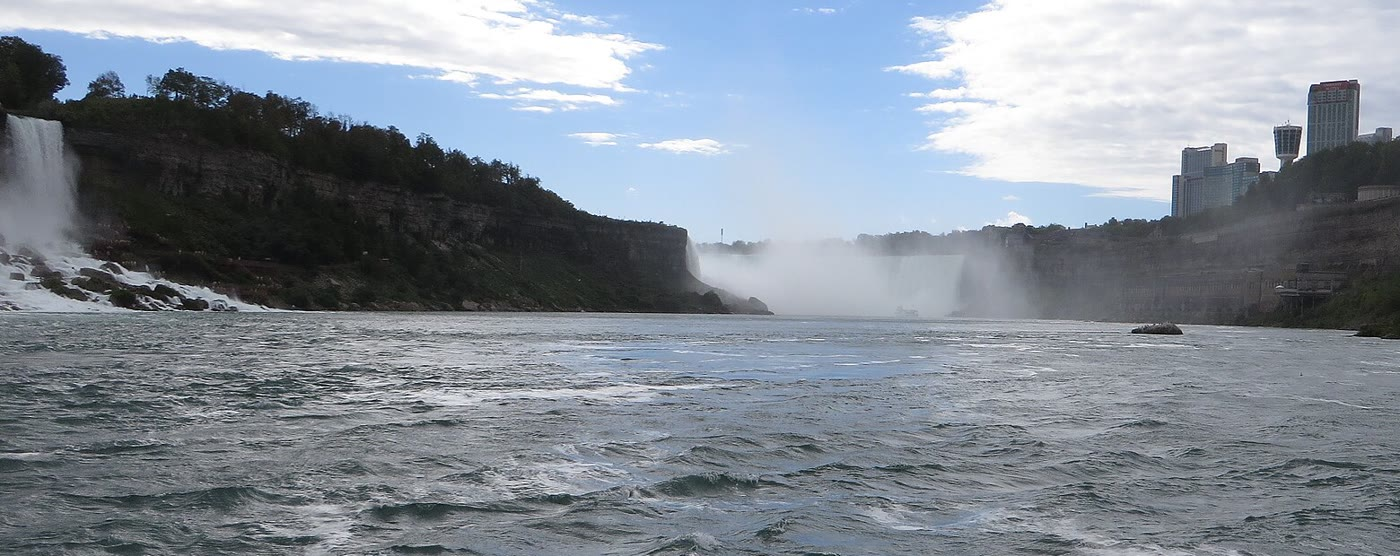
\includegraphics[width=\linewidth]{images/book5/b3-niagara-gorge.jpg}

{\scriptsize 尼亚加拉峡谷，朝上游望去是
笼罩在水雾中的马蹄瀑布，左缘为美国瀑布。照片：Ken Lund,
CC BY-SA 2.0（裁剪）。}
\end{minipage}
\end{inthefield}
% ledger: ijc18:niagara, photo:b3-niagara-gorge


\section{冰川侵蚀}\label{sec:b3:quantitative-geomorphology:glacial}

冰川沿其床面滑动（底部滑动，
见第~\ref{ch:b3:glaciology}~章），以磨蚀方式侵蚀床面：冰中携带的碎屑刮擦岩石，
并以拔蚀方式拖出被
裂隙松动的岩块。两者均随滑动速度增大。

\begin{definition}[冰川侵蚀定律]\label{def:b3:quantitative-geomorphology:glacial}
\emph{冰川侵蚀定律}\index{冰川侵蚀定律}给出冰川床面的侵蚀速率，
即 $E = K_G\,u_s^{\,l}$，其中 $u_s$ 为
滑动速度，$K_G$ 为系数，$l$ 为指数。
\end{definition}

地貌模型通常取 $l = 1$，实际采用的值介于 1 与 2 之间。
对 38 条冰川的汇总发现，其侵蚀速率跨越五个
数量级，侵蚀与滑动速度相关，其中 $l = 0.65$，
$K_G = 10^{-4}$（$E$ 以米每年计）；侵蚀最快的是在温冰川之下，
温冰川由大量降雪补给，滑动迅速。冰层在谷轴处最厚、流速最快，
因此谷底比两侧下切得更多，
山谷便呈 U 形。
% ledger: cook20:glacial

\begin{definition}[冰川锯效应]\label{def:b3:quantitative-geomorphology:buzzsaw}
\emph{冰川锯效应}\index{冰川锯效应}是冰川对
山脉高度所设的上限：凡岩石升至冰川形成的海拔之上，
冰川便以与其抬升相同的速率侵蚀它，无论抬升速率大小，
使山峰与平均海拔都聚集在该海拔附近。
\end{definition}

\section{构造与侵蚀}\label{sec:b3:quantitative-geomorphology:tectonics}

\begin{definition}[地形稳态]\label{def:b3:quantitative-geomorphology:steady-state}
若某地貌处于\emph{地形稳态}\index{地形稳态}，
即其侵蚀速率处处等于岩石抬升速率，
从而其高程不变，尽管岩石仍在穿过它。
\end{definition}

用不同时间跨度测得的速率可以检验这一状态。\omterm{def:b3:advanced-geochronology:cosmogenic}{宇宙成因
核素}取自河砂，给出流域在剥去一层岩石所需时间内的平均侵蚀速率，
该岩层厚度约为其产生的衰减长度的量级，
即约 \qty{55}{cm} 的岩石；\omterm{def:b3:orogenic-wedges:thermochronology}{热年代计}及其\omterm{def:b3:orogenic-wedges:age-elevation}{年龄–高程关系}给出
数百万年尺度上的折返速率。若二者彼此一致，
且与抬升速率相符，则该地貌很可能处于\omterm{def:b3:quantitative-geomorphology:steady-profile}{稳态}；若
短期速率在下游高于上游，
则说明有\omterm{def:b3:quantitative-geomorphology:knickpoint}{裂点}正在经过。移走岩石还会使岩石圈卸载，
岩石圈随之回升。
% ledger: zech04:exposure

\begin{definition}[剥蚀均衡回弹]\label{def:b3:quantitative-geomorphology:rebound}
\emph{剥蚀均衡回弹}\index{剥蚀均衡回弹}是
处于地壳均衡状态的区域岩石表面的抬升，
对侵蚀所移除质量的响应。
\end{definition}

\begin{proposition}[谷地加深，山峰抬升]\label{prop:b3:quantitative-geomorphology:rebound}
在艾里均衡中，密度为 $\rho_c$ 的地壳位于密度为 $\rho_m$ 的地幔之上，
从某区域移除平均厚度为 $\bar e$ 的地壳，将整个区域抬升
$(\rho_c/\rho_m)\,\bar e$。若侵蚀仅限于谷地，
未被侵蚀的山顶抬升同样的量，而平均地表
仅下降 $(1 - \rho_c/\rho_m)\,\bar e$。
\end{proposition}

\begin{proof}
均衡补偿要求固定深度以上每个柱体的质量保持不变。
若移除厚度为 $\bar e$ 的地壳并在补偿区域上取平均，
则单位面积质量减少 $\rho_c \bar e$；
补偿这部分需要地幔在深处流入，使柱体底部
及其上的一切抬升 $\delta$，满足 $\rho_m \delta = \rho_c \bar
e$。未失去岩石的山顶抬升 $\delta$，平均地表
失去 $\bar e$，又得到 $\delta$。
\end{proof}

参考地球模型中地壳的厚度加权密度为
\qty{2.72}{g/cm^3}，莫霍面以下地幔的密度为 \qty{3.38}{g/cm^3}，
两者之比为 0.80：每侵蚀一百米岩石，平均地表
仅下降二十米。古老高原的深切因此可使其山顶抬升，
即使高原本身仍在被削低。
% ledger: prem:crust-mantle-ratio

\begin{omfigure}
\begin{tikzpicture}[x=0.6cm, y=0.6cm, font=\scriptsize]
\begin{scope}
\fill[omDef!12] (0,0) rectangle (8,4);
\draw[thick] (0,4) -- (8,4);
\draw[densely dashed] (0,0) -- (8,0);
\node[anchor=north] at (4,-0.1) {地壳底部};
\node at (4,2) {地壳 $\rho_c$};
\node at (4,-1.2) {地幔 $\rho_m$};
\node[anchor=south] at (4,4.1) {侵蚀前};
\end{scope}
\begin{scope}[xshift=6.2cm]
\fill[omDef!12] (0,0.8) -- (0,4.8) -- (1.4,4.8) -- (2.0,2.4) -- (2.6,4.8) -- (5.4,4.8) -- (6.0,2.4) -- (6.6,4.8) -- (8,4.8) -- (8,0.8) -- cycle;
\draw[thick] (0,4.8) -- (1.4,4.8) -- (2.0,2.4) -- (2.6,4.8) -- (5.4,4.8) -- (6.0,2.4) -- (6.6,4.8) -- (8,4.8);
\draw[black!50, densely dashed] (0,4) -- (8,4);
\draw[densely dashed] (0,0.8) -- (8,0.8);
\draw[densely dashed, black!40] (0,0) -- (8,0);
\draw[<->, omThm] (8.3,4.05) -- (8.3,4.75) node[midway, right] {$\delta$};
\draw[<->, omThm] (8.3,0.05) -- (8.3,0.75) node[midway, right] {$\delta$};
\node[anchor=west, font=\scriptsize] at (8.1,2.4) {$\delta = (\rho_c/\rho_m)\,\bar e$};
\node[anchor=south] at (4,5.0) {谷地下切之后};
\node[anchor=north] at (2.0,2.3) {谷地};
\end{scope}
\end{tikzpicture}

\par\smallskip{\small \omterm{def:b3:quantitative-geomorphology:rebound}{剥蚀均衡回弹}示意图。切割
河谷移去了平均厚度为 $\bar e$ 的地壳，此柱体
在其底部及未被切割的山顶处各抬升 $\delta = (\rho_c/\rho_m)\bar e$，
（灰色虚线为原地表）。}\label{fig:b3:quantitative-geomorphology:rebound}
\end{omfigure}

\section{练习}

\begin{exercise}[$\star$]\label{exo:b3:quantitative-geomorphology:1}
一个海岸陡坎的错距为 \qty{4}{m}（$a = \qty{2}{m}$），位于一片
远场斜坡（坡度为 0.04）之上，其最大梯度现为 0.30。求
$\kappa t$，再用 $\kappa = \qty{5e-3}{m^2/\text{年}}$ 求该陡坎的年龄。
\end{exercise}
% ledger: whipple04:scarp-erf, whipple04:scarp-kappa

\begin{exercise}[$\star$]\label{exo:b3:quantitative-geomorphology:2}
一次激光雷达测量给出一处位于山脊上的山顶，其曲率为 \qty{-0.012}{m^{-1}}，
该山脊的扩散率为 \qty{4e-3}{m^2/\text{年}}。求其侵蚀速率（单位
\unit{mm/\text{年}}），并求山顶与相距
\qty{80}{m} 的河道之间的起伏高差，假设处于\omterm{def:b3:quantitative-geomorphology:steady-profile}{稳态}。
\end{exercise}

\begin{exercise}[$\star$]\label{exo:b3:quantitative-geomorphology:3}
取 $m = 0.5$，$n = 1$，$K = \qty{2e-6}{\text{年}^{-1}}$，求
一条汇水面积为 \qty{25}{km^2}、坡度为 0.01 的河流的下切速率。
$K$ 在一般的 $m$ 和 $n$ 情形下的单位是什么？
\end{exercise}

\begin{exercise}[$\star$]\label{exo:b3:quantitative-geomorphology:4}
三条河流出现\omterm{def:b3:quantitative-geomorphology:knickpoint}{裂点}：（a）砂岩岩层穿过切割页岩形成的河谷之处；
（b）河流穿过活动正断层，自下盘流向上盘之处；
（c）某一流域内所有河流在大致相同的高程处出现\omterm{def:b3:quantitative-geomorphology:knickpoint}{裂点}，
这一高程位于海岸上方数千米处，该海岸
因一次地震而抬升。哪些\omterm{def:b3:quantitative-geomorphology:knickpoint}{裂点}是固定的，哪些将会迁移？
\end{exercise}

\begin{exercise}[$\star\star$]\label{exo:b3:quantitative-geomorphology:5}
取 $m = 1$，$n = 2$，求 $\theta$ 及\omterm{def:b3:quantitative-geomorphology:steady-profile}{稳态}梯度，其中 $A =
\qty{10}{km^2}$、$U = \qty{0.1}{mm/\text{年}}$，且 $K = 10^{-9}$（以米和
年为单位）。
若 $U$ 加倍，陡峭度将变为原来的多少倍？与 $n =
1$ 的情形相比较。
\end{exercise}

\begin{exercise}[$\star\star$]\label{exo:b3:quantitative-geomorphology:6}
河流的汇水面积随距分水岭距离 $d$ 增长，满足 $A =
c\,d^{h}$。证明：自出口（位于 $d = L$）向上游量度时，
\[
\chi(d) = \frac{A_0^{\theta}}{c^{\theta}}\,\frac{L^{p} - d^{p}}{p},
\qquad p = 1 - h\theta ,
\]
并取 $c = 2$（SI 单位制）、$h = 1.8$、$\theta = 0.45$、$A_0 =
\qty{1}{km^2}$、$L = \qty{20}{km}$ 与 $d = \qty{5}{km}$，计算该值。
\end{exercise}

\begin{exercise}[$\star\star$]\label{exo:b3:quantitative-geomorphology:7}
取 $n = 1$、$m = 0.5$、$K = \qty{2e-6}{\text{年}^{-1}}$，求
汇水面积为 $A = \qty{100}{km^2}$ 处\omterm{def:b3:quantitative-geomorphology:knickpoint}{裂点}的传播速度（单位为 m/ka），以及
以该速度传播 \qty{5}{km} 所需的时间。
实际上为何需要更长时间？
\end{exercise}

\begin{exercise}[$\star\star$]\label{exo:b3:quantitative-geomorphology:8}
一片高原上切入了深 \qty{600}{m} 的河谷，平均占高原面积的
\qty{40}{\percent}。取 $\rho_c/\rho_m = 0.80$，求
平均剥蚀厚度、山顶的抬升量以及
平均高程的变化。
\end{exercise}
% ledger: prem:crust-mantle-ratio

\begin{exercise}[$\star\star$]\label{exo:b3:quantitative-geomorphology:9}
\omterm{def:b3:quantitative-geomorphology:soil-production}{土壤生成函数}中 $P_0 = \qty{0.3}{mm/\text{年}}$，$h_0 =
\qty{0.5}{m}$。求侵蚀速率为
\qty{0.05}{mm/\text{年}} 和 \qty{0.2}{mm/\text{年}} 时的\omterm{def:b3:quantitative-geomorphology:steady-profile}{稳态}土层厚度。侵蚀速率为
\qty{0.4}{mm/\text{年}} 时会发生什么？
\end{exercise}

\begin{exercise}[$\star\star\star$]\label{exo:b3:quantitative-geomorphology:10}
一座处于\omterm{def:b3:quantitative-geomorphology:steady-profile}{稳态}的山丘以 $E = \qty{0.1}{mm/\text{年}}$ 的速率被侵蚀，$\kappa =
\qty{5e-3}{m^2/\text{年}}$，采用\omterm{def:b3:quantitative-geomorphology:critical}{临界坡度}的非线性定律，并取练习中的
$S_c = 1.2$。证明：距分水岭 $x$ 处的通量为
$E x$，解出梯度，并计算在 20、50、100 和
\qty{200}{m} 处的梯度，并与线性扩散相比较。
描述该山丘的形态。
\end{exercise}

\begin{exercise}[$\star\star\star$]\label{exo:b3:quantitative-geomorphology:11}
证明：对于 $n = 1$，河网对出口处变化的响应时间为
$\chi_h/(K A_0^m)$，其中 $\chi_h$ 为
河道源头处 $\chi$ 的最大值。对图中上游河流计算该时间，
（$A_0 = \qty{1}{km^2}$、$m = 0.5$、$K = \qty{e-6}{\text{年}^{-1}}$），先仅针对其
干流计算，其源头处 $\chi = \qty{5464}{m}$，再针对整个河网计算，
其最高源头位于支流 1 上，$\chi = \qty{7237}{m}$。
\end{exercise}

\begin{exercise}[$\star\star\star$]\label{exo:b3:quantitative-geomorphology:12}
在 $n = 1$ 且 $U$ 均匀的河网中，某一支流流经的岩石可蚀性
为其余河段的两倍（$2K$），该段位于汇入点 $\chi_j$ 以上。证明：
该支流在 $(\chi, z)$ 平面上的\omterm{def:b3:quantitative-geomorphology:steady-profile}{稳态}直线斜率
为干流在 $\chi_j$ 以上部分斜率的一半；并证明：自出口产生的\omterm{def:b3:quantitative-geomorphology:knickpoint}{裂点}
当干流\omterm{def:b3:quantitative-geomorphology:knickpoint}{裂点}位于 $\chi_k > \chi_j$ 处时，到达该支流上
$\chi = \chi_j + 2(\chi_k - \chi_j)$ 的点。
\end{exercise}

\section{问题：瓦尔登河的瀑布}

\begin{problem}[{周末问题——一条虚构高地河流的剖面、陡峭度与
可蚀性，以及其瀑布的年龄}]
\label{pb:b3:quantitative-geomorphology:1}
瓦尔登丘陵以西，河流先流经一片由片岩构成的高地，
在西缘处进入图幅，海拔为 \qty{170}{m}。此点即其出口，
其上游的干流自分水岭起算长 \qty{12}{km}，
汇水面积为 $A = 4.5\,d^{1.7}$（\unit{m^2}，$d$ 为距分水岭的
距离，单位为米），河道源头位于 $d = \qty{300}{m}$ 处。取岩石
隆升速率，取为瓦尔登河流域的剥蚀速率，该速率由其
在本科一年级分册中的负荷量求得，为 \qty{43}{m/Ma}。取 $n = 1$，参考面积 $A_0 = \qty{1}{km^2}$。
干流上一座高 \qty{25}{m} 的瀑布，位于出口上游
\qty{4.60}{km} 处。所有数值均为虚构。

\medskip\noindent\textbf{第一部分——剖面。}
\begin{enumerate}
\item 计算出口处与河道源头处的汇水面积。
\item 在长 \qty{200}{m} 的河段上测得的坡度，这些河段远离
  瀑布：

  \smallskip
  {\small\begin{tabular}{l*{6}{c}}
  $A$ (\unit{km^2}) & 0.388 & 0.587 & 0.888 & 1.345 & 2.036 & 3.082 \\
  $S$ & 0.06641 & 0.05026 & 0.04888 & 0.03322 & 0.03688 & 0.02688 \\[2pt]
  $A$ (\unit{km^2}) & 4.665 & 7.061 & 10.69 & 16.18 & 24.49 & 37.08 \\
  $S$ & 0.01921 & 0.01713 & 0.01545 & 0.01419 & 0.007922 & 0.007855
  \end{tabular}}

  \smallskip
  根据首、末两点估算\omterm{def:b3:quantitative-geomorphology:indices}{凹度指数}。
\item $\log S$ 对 $\log A$ 的最小二乘斜率为 $-0.466$。
  它与 $\theta = 0.5$ 是否一致？
\item 取 $\theta_{\mathrm{ref}} = 0.5$，计算第一点和最后一点的 $k_{sn} = S A^{0.5}$（$A$ 以
  \unit{m^2} 计，并说明
  十二个值的几何平均值 \qty{45.1}{m} 代表什么。
\item 为什么坡度的离散程度远大于高程？
\item 利用 χ 分析练习中的公式，计算 $\chi$ 在 $d =
  \qty{9.00}{km}$ 处，该点位于瀑布下方。
\end{enumerate}

\medskip\noindent\textbf{第二部分——陡度与可侵蚀性。}
\begin{enumerate}[resume]
\item 河流在 $d = \qty{9.00}{km}$ 处的高程为 \qty{193.4}{m}。请计算
  瀑布下方 χ 图的斜率以及陡度 $k_{sn}$。
\item 在 $k_{sn}$ 的两种估计中，你会更信任哪一种，
  是这里的估计，还是坡度–面积法的估计？为什么？
\item 假设瀑布下方处于\omterm{def:b3:quantitative-geomorphology:steady-profile}{稳态}，由
  隆升速率计算 $K$。
\item 检验出口处的下切速率（其坡度为
  0.00691）是否等于隆升速率。
\item 计算出口处及瀑布处\omterm{def:b3:quantitative-geomorphology:knickpoint}{裂点}的
  波速，单位为 m/ka。
\item 计算\omterm{def:b3:quantitative-geomorphology:steady-profile}{稳态}剖面上河道源头的高程，以及
  主干河道的地形起伏。
\end{enumerate}

\medskip\noindent\textbf{第三部分——瀑布。}
\begin{enumerate}[resume]
\item 当 $n = 1$ 时，为什么瀑布仍保持
  与\omterm{def:b3:quantitative-geomorphology:knickpoint}{侵蚀基准面}下降量相同的高度？
\item 计算瀑布处的 $\chi$。
\item 计算\omterm{def:b3:quantitative-geomorphology:knickpoint}{裂点}从出口移动到
  现在位置所用的时间。
\item 再过 \qty{300}{ka}，\omterm{def:b3:quantitative-geomorphology:knickpoint}{裂点}将位于何处？
\item 支流 3 在出口上游 \qty{2.5}{km} 处汇入主干；
  该支流长 \qty{5}{km}，$A = 1.5\,s^{1.7}$（$s$ 自其自身分水岭起算）。
  其瀑布应位于何处？
\item 支流 1 和支流 2 分别在出口上游 8 和 \qty{5}{km}
  处汇入主干。试说明它们为何没有瀑布。
\end{enumerate}

\medskip\noindent\textbf{第四部分——坡面与年龄。}
\begin{enumerate}[resume]
\item 瀑布上方的激光雷达测量给出山顶曲率为
  \qty{-0.0086}{m^{-1}}。取 $\kappa = \qty{5e-3}{m^2/\text{年}}$，计算
  侵蚀速率，并与隆升速率作比较。
\item 坡面长约 \qty{150}{m}。比较其响应时间
  $L^2/\kappa$ 与第三部分中求得的年龄。
\item 描述瀑布下方坡面的现状，以及它们将如何
  变化。
\item 隆升速率的不确定度为 \qty{20}{\percent}。给出
  年龄的取值范围。
\item 若 $n$ 为 2，瀑布会如何演化？
\item 给出\omterm{def:b3:quantitative-geomorphology:knickpoint}{侵蚀基准面}下降的年龄。
\end{enumerate}
\end{problem}
% ledger: whipple04:steepness, whipple04:scarp-kappa
